\documentclass{article}

\usepackage[utf8]{inputenc}
\usepackage[turkish, shorthands = :!]{babel}
\usepackage[T1]{fontenc}
\usepackage{lmodern}

\usepackage{fancyhdr, mathtools, comment}

\usepackage{tikz} % PGF is a macro package for creating graphics. It is platform- and format-independent and works together with the most important TeX backend drivers, including pdfTeX and dvips. It comes with a user-friendly syntax layer called TikZ.
\usetikzlibrary{patterns} % taralı alanlar için

\usepackage{pgfplots} % Create normal/logarithmic plots in two and three dimensions
\pgfplotsset{compat = 1.18} % eski belgelerin görünümünü bozmadan pgfplots paketini güncel tutmak için

\begin{comment}
Normalde ark çizimi tikzpicture'da şu şekilde yapılıyor:
	\draw (x, y) arc (alfa : beta : r);
Burada (x, y) arkın başladığı nokta, alfa ve beta derece cinsinden arkın başlangıç ve bitiş açısı, r arkın yarıçapı. Arkı, başladığı noktayı değil de, ilişkili çemberin merkezini vererek çizdirmek istersek basit bir dönüşüm yapmamız yeterli: (x0, y0) çemberin merkezi ise arkın başladığı nokta
	(x0 + r*cos(alfa), y0 + r*sin(alfa))
olacak. Aşağıdaki komut tam da bu dönüşümü gerçekleştirmeye yarıyor; yani çemberin merkezi, yarıçapı ve arkın başlangıç açısı verildiğinde arkın başlangıç noktasını döndürüyor:
	\centertostart{x0}{y0}{r}{alfa} = (x0 + r*cos(alfa), y0 + r*sin(alfa)) = (x, y).
\end{comment}

\newcommand{\centertostart}[4]{({#1 + #3*cos(#4)}, {#2 + #3*sin(#4)})}

\renewcommand{\headrulewidth}{0 pt}
\pagestyle{fancy}
\fancyhf{}
\fancyhead[C]{\thepage}

\begin{document}

%%%%%%% SAYFA 1 %%%%%%%

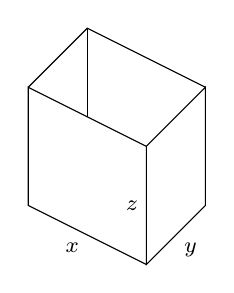
\begin{tikzpicture}[scale = 0.75]
\begin{footnotesize} % aşağıdaki x, y, z'nin yazı tipi boyutunu küçültmek için
\draw (0, 0) -- (1, 1) -- (1, 3) -- (0, 2) -- cycle;
%\draw (0, 0) -- (1, 1) -- (1, 3) -- (0, 2) -- (0, 0); % alternatif yazım
\draw (0, 0) -- (-2, 1) -- (-2, 3) -- (0, 2);
\draw (-2, 3) -- (-1, 4) -- (1, 3);
\draw (-1, 4) -- (-1, 2.5);
\node [below left] at (-1, 0.5) {$x$};
\node [below right] at (0.5, 0.5) {$y$};
\node [left] at (0, 1) {$z$};
\end{footnotesize}
\end{tikzpicture}

\bigskip
\hrule
\bigskip

\begin{tikzpicture}
\draw [help lines, dashed] (0, 0) grid (4, 2); % yardımcı çizgileri eksenlerden önce çizmeli
% eksenler
\draw [->] (-1, 0) -- (5, 0) node [right] {Zaman (dk)};
\draw [->] (0, -1) -- (0, 3) node [above] {Yol (km)};
% alternatif yazım
%\draw [->] (-1, 0) -- (5, 0);
%\draw [->] (0, -1) -- (0, 3);
%\node [right] at (5, 0) {Zaman (dk)};
%\node [above] at (0, 3) {Yol (km)};
\node [below left] at (0, 0) {0};
\foreach \i in {1, ..., 4}
	\node [below] at (\i, 0) {\i};
\foreach \i in {1, 2}
	\node [left] at (0, \i) {\i};
% grafik
\draw [thick, domain = 0 : 4, samples = 100] plot (\x, {sqrt(\x)}); % sqrt(\x) ifadesini askı parantez içine almazsak hata veriyor
\end{tikzpicture}

\bigskip
\hrule
\bigskip

\begin{tikzpicture}
% eksenler
\draw [->] (-4.5, 0) -- (5, 0) node [right] {$x$};
\draw [->] (0, -2.5) -- (0, 3.5) node [above] {$y$};
\draw (-4, -0.1) grid (4, 0.1); % düzlem boyunca uzanan bir ızgara (grid) düşünelim; bunun sadece (-4, -0.1) ve (4, 0.1) noktalarının belirlediği dikdörtgen bölgeyle kesişimini çizdiriyoruz (aynı sonucu bir için döngüsü kullanarak da elde edebilirdik; bk. bir sonraki örnek)
\draw (-0.1, -2) grid (0.1, 2);
\node [below left] at (-0.1, -0.1) {0};
\foreach \i in {1, ..., 4}
	\node [below] at (\i, -0.1) {\i};
\foreach \i in {1, 2}
	\node [left] at (-0.1, \i) {\i};
% grafik
\draw [thick, domain = -4 : 4, samples = 100] plot (\x, {4*\x / (\x*\x + 1)}); % y = 4x/(x² + 1)
\node [above right] at (1, 2) {$y = \dfrac{4x}{x^2 + 1}$};
\end{tikzpicture}

\newpage

%%%%%%% SAYFA 2 %%%%%%%

\begin{tikzpicture}
% eksenler
\draw [->] (-1.5, 0) -- (4, 0) node [right] {$x$};
\draw [->] (0, -0.5) -- (0, 3) node [above] {$y$};
\node [below left] at (0, 0) {0};
\draw (-1, 0) -- (-1, 0.15);
\node [below] at (-1, 0) {-1};
\foreach \i in {1, 2, 3}
{
	\draw (\i, 0) -- (\i, 0.15);
	\node [below] at (\i, 0) {\i};
}
\foreach \i in {1, 2}
{
	\draw (0, \i) -- (0.15, \i);
	\node [left] at (0, \i) {\i};
}
% grafikler
\draw [thick, domain = -1 : 0] plot (\x, -\x); % y = -x
\draw [thick, domain = 0 : 1] plot (\x, 2*\x*\x); % y = 2x²
\draw [thick, domain = 1 : 2] plot (\x, 1);
\draw [thick, domain = 2 : 3] plot (\x, 1);
\filldraw (-1, 1) circle (2 pt); % 2 pt yarıçaplı içi dolu çember
\filldraw (1, 1) circle (2 pt);
\filldraw (2, 2) circle (2 pt);
\filldraw (3, 1) circle (2 pt);
\filldraw [fill = white] (1, 2) circle (2 pt);
\filldraw [fill = white] (2, 1) circle (2 pt);
\end{tikzpicture}

\bigskip
\hrule
\bigskip

\begin{tikzpicture}
% eksenler
\draw [->] (0, -3) -- (0, 3) node [right] {$x$};
\draw [->] (-3, 0) -- (3, 0) node [above] {$y$};
% grafikler
\draw [thick, domain = -2.5 : 1.5, dash dot] plot (\x, 2^\x); % f(x) = 2^x
\draw [thick, domain = -2.5 : 2.5] plot (\x, \x); % g(x) = x
\draw [thick, domain = -1.35 : 1.35, dashed] plot (\x, \x*\x*\x); % h(x) = x³
\node [above right] at (-2.5, 0.2) {$f$};
\node [above] at (-2.5, -2.5) {$g$};
\node [above right] at (-1.35, -2.5) {$h$};
\end{tikzpicture}

\newpage

%%%%%%% SAYFA 3 %%%%%%%

\begingroup
\renewcommand \pi {3.141593} % pi sayısı
\begin{tikzpicture}[scale = 0.5, declare function = {
	f1(\x) = 2*\x + 2;			% y = 2x + 2
	f2(\x) = \x*\x;				% y = x²
	f3(\x) = 4*\x / (\x*\x + 1); 	% y = 4x/(x² + 1)
	f4(\x) = \x^3; 				% y = x³
	f5(\x) = 2^\x; 				% y = 2^x
	f6(\x) = exp(\x); 			% y = e^x
	f7(\x) = ln(\x); 				% y = ln(x)
	f8(\x) = sin((360/(2*\pi))*\x);	% y = sin(x)
	f9(\x) = cos((360/(2*\pi))*\x); % y = cos(x)
	f10(\x) = sqrt(\x);			% y = x^{1/2}
}]
\draw [help lines, dashed] (-8, -8) grid (8, 8);
% eksenler
\draw [->] (-8, 0) -- (8, 0);
\draw [->] (0, -8) -- (0, 8);
% grafik
\draw [thick, domain = -5 : 3, samples = 100] plot (\x, {f1(\x)}); % f1(\x) ifadesini askı parantez içine almazsak hata veriyor
\draw [thick, domain = -2.83 : 2.83, samples = 100] plot (\x, {f2(\x)});
\draw [thick, domain = -8 : 8, samples = 100] plot (\x, {f3(\x)});
\draw [thick, domain = -2 : 2, samples = 100] plot (\x, {f4(\x)});
\draw [thick, domain = -8 : 3, samples = 100] plot (\x, {f5(\x)});
\draw [thick, domain = -8 : 2.08, samples = 100] plot (\x, {f6(\x)});
\draw [thick, domain = 0.001 : 8, samples = 100] plot (\x, {f7(\x)});
\draw [thick, domain = -8 : 8, samples = 100] plot (\x, {f8(\x)});
\draw [thick, domain = -8 : 8, samples = 100] plot (\x, {f9(\x)});
\draw [thick, domain = 0 : 8, samples = 100] plot (\x, {f10(\x)});
\end{tikzpicture}
\endgroup

\bigskip
\hrule
\bigskip

\begingroup % böyle gruplamazsak, aşağıda \c komutunun tanımını değiştirdiğimiz için, akabinde ç ve ş harfleri yanlış basılıyor
\newcommand \e {2.718281} % Euler sabiti
\renewcommand \a {10}
\renewcommand \c {-5}
\begin{tikzpicture}[scale = 0.5, declare function = {
	f(\x) = \a*(\e^(\x / \a) + \e^(-\x / \a))/2 + \c; % f(x) = a*cosh(x/a) + c
}]
% eksenler
\draw [->] (-10, 0) -- (10, 0) node [right] {$x$};
\draw [->] (0, 0) -- (0, 10) node [above] {$y$};
\node [below] at (0, 0) {0};
% grafik
\draw [thick, domain = -8 : 8, samples = 100] plot (\x, {f(\x)}) node [above] {$y = a \cosh(x/a) + c$};
\filldraw (8, {f(8)}) circle (4 pt);
\filldraw (-8, {f(-8)}) circle (4 pt);
\draw [dashed] (8, {f(8)}) -- (8, 0) node [below] {$x_0$};
\draw [dashed] (-8, {f(-8)}) -- (-8, 0) node [below] {$-x_0$};
\node [below left] at (0, 5) {$b$};
\draw (-0.1, {f(8)}) -- (0.1, {f(8)});
\node [left] at (0, {f(8)}) {$y_0$};
\end{tikzpicture}
\endgroup

\newpage

%%%%%%% SAYFA 4 %%%%%%%

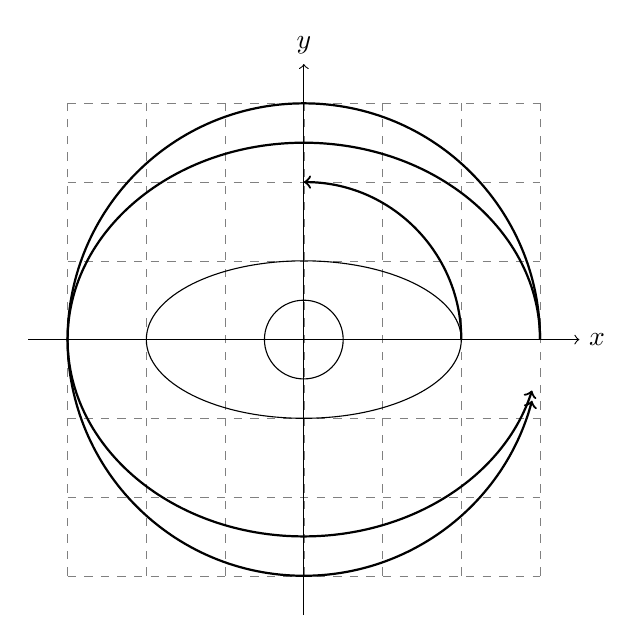
\begin{tikzpicture}
\draw [help lines, dashed] (-3, -3) grid (3, 3);
% eksenler
\draw [->] (-3.5, 0) -- (3.5, 0) node [right] {$x$};
\draw [->] (0, -3.5) -- (0, 3.5) node [above] {$y$};
% çemberler ve elipsler
\draw (0, 0) circle (0.5); % orijin merkezli 0.5 yarıçaplı çember
\draw (0, 0) circle (2 and 1); % büyük yarıçapı 2, küçük yarıçapı 1 olan orijin merkezli elips
%\draw (0, 0) ellipse [x radius = 2, y radius = 1]; % alternatif yazım
% arklar
\draw [->, thick] (2, 0) arc (0 : 90 : 2); % 2 yarıçaplı çemberde 0°'den 90°'ye uzanan ark, başlangıç noktası (2, 0)
%\draw [->, thick] \centertostart{0}{0}{2}{0} arc (0 : 90 : 2); % aynı arkın \centertostart komutuyla çizimi
\draw [->, thick] (3, 0) arc (0 : 345 : 3); % 3 yarıçaplı çemberde 0°'den 345°'ye uzanan ark, başlangıç noktası (3, 0)
\draw [->, thick] (3, 0) arc (0 : 345 : 3 and 2.5); % yarıçapları 3 ve 2.5 olan elipste 0°'den 345°'ye uzanan eliptik ark, başlangıç noktası (3, 0)
% 0°'den başlamazsak çemberden elipse geçişte üstten ve alttan aynı oranda sıkışma olmuyor:
%\draw [->, thick] (0, 3) arc (90 : 345 : 3); % 3 yarıçaplı çemberde 90°'den 345°'ye uzanan ark, başlangıç noktası (0, 3)
%\draw [->, thick] (0, 3) arc (90 : 345 : 3 and 2.5);
\end{tikzpicture}

\bigskip
\hrule
\bigskip

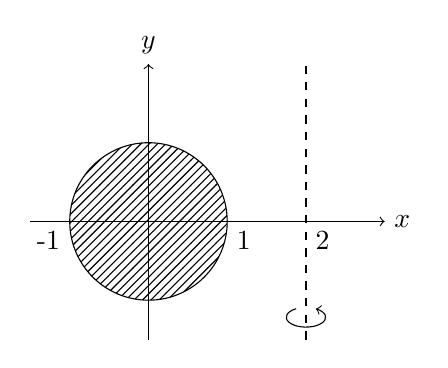
\begin{tikzpicture}
% eksenler
\draw [->] (-1.5, 0) -- (3, 0) node [right] {$x$};
\draw [->] (0, -1.5) -- (0, 2) node [above] {$y$};
% disk
\filldraw [pattern = north east lines] (0, 0) circle (1);
\node [below left] at (-1, 0) {-1};
\node [below right] at (1, 0) {1};
% döndürme ekseni
\draw [dashed] (2, -1.5) -- (2, 2);
\node [below right] at (2, 0) {2};
\draw [->] \centertostart{2}{-1.325}{0.25}{120} arc (120 : 420 : 0.25 and 0.125);
% \centertostart'sız yazacak olsaydık: \draw [->] ({2 + 0.25*cos(120)}, {-1.325 + 0.25*sin(120)}) arc (120 : 420 : 0.25 and 0.125);
\end{tikzpicture}

\bigskip
\hrule
\bigskip

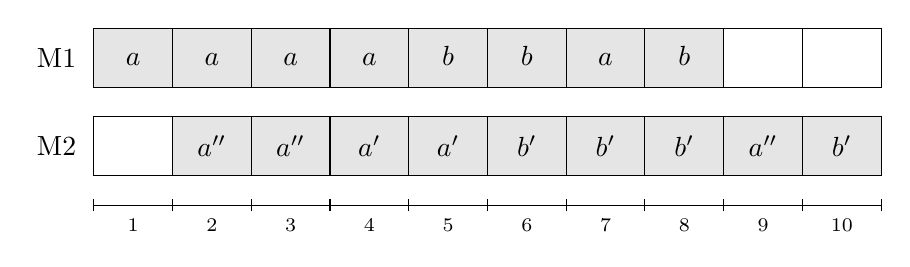
\begin{tikzpicture}[xscale = 1, yscale = 0.75]
% legend
\draw (0, -0.1) grid (10, 0.1);
\begin{scriptsize}
\foreach \i in {1, ..., 10}
	\node [below] at (\i - 0.5, -0.1) {\i};
\end{scriptsize}
\node [left] at (-0.1, 1) {M2};
\node [left] at (-0.1, 2.5) {M1};
% boxes
\fill [black!10] (1, 0.5) rectangle (10, 1.5);
\fill [black!10] (0, 2) rectangle (8, 3);
\foreach \i in {0, ..., 9}
{
	\draw (\i, 0.5) rectangle (\i + 1, 1.5);
	\draw (\i, 2) rectangle (\i + 1, 3);
}
% items
\foreach \i in {0.5, 1.5, 2.5, 3.5, 6.5} { \node [above] at (\i, 2.2) {$a$}; }
\foreach \i in {4.5, 5.5, 7.5} { \node [above] at (\i, 2.2) {$b$}; }
\foreach \i in {3.5, 4.5} { \node at (\i, 1) {$a'$}; }
\foreach \i in {1.5, 2.5, 8.5} { \node at (\i, 1) {$a''$}; }
\foreach \i in {5.5, 6.5, 7.5, 9.5} { \node at (\i, 1) {$b'$}; }
\end{tikzpicture}

\newpage

%%%%%%% SAYFA 5 %%%%%%%

\begingroup
\newcommand \thickness {0.2} % merdivenin kalınlığı
\begin{tikzpicture}
% eksenler
\draw [->] (-0.5, 0) -- (5, 0) node [right] {$x$};
\draw [->] (0, 0) -- (0, 4) node [above] {$y$};
\node [below] at (0, 0) {0};
% merdiven
\draw [fill = black!20, rotate around = {-36.8699 : (4, 0)}] (-1, 0) rectangle (4, \thickness); % (-1, 0) ve (4, \thickness) noktalarının belirlediği dikdörtgeni (4, 0) noktasını merkez alarak saat yönünde arccos(4/5) = 36.8699° döndürüyoruz
\foreach \i in {0, ..., 6}
	\fill [rotate around = {-36.8699 : (4, 0)}] (-0.9 + 0.8*\i, 0.5*\thickness) circle (1 pt); % [-0.9, 3.9] arasında 0.8 aralıklı yedi nokta çizilmesi
\node [right] at (2, 2) {merdiven};
% x(t), y(t) ve oklar
\node [below] at (4, 0) {$x(t)$};
\draw [->, very thick] (4, 0) -- (4.5, 0);
\node [left] at (0, 3) {$y(t)$};
\draw [->, very thick] (0, 3) -- (0, 2.5);
\end{tikzpicture}
\endgroup

\bigskip
\hrule
\bigskip

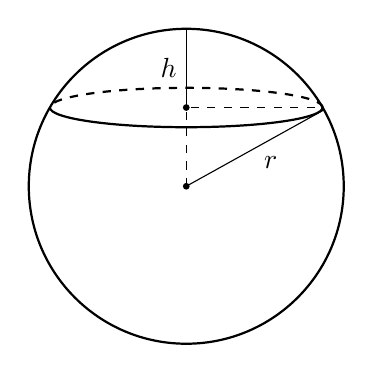
\begin{tikzpicture}
\draw [thick] (0, 0) circle (2);
\draw [thick] ({sqrt(3)}, 1) arc (0 : -180 : {sqrt(3)} and 0.25);
\draw [thick, dashed] ({sqrt(3)}, 1) arc (0 : 180 : {sqrt(3)} and 0.25);
\draw (0, 1) -- (0, 2);
\draw (0, 0) -- ({sqrt(3) + 0.025}, 1 - 0.025);
\draw [dashed] (0, 0) -- (0, 1) -- ({sqrt(3)}, 1);
\filldraw (0, 0) circle (1 pt);
\filldraw (0, 1) circle (1 pt);
\node [below right] at ({sqrt(3)/2}, 0.5) {$r$};
\node [left] at (0, 1.5) {$h$};
\end{tikzpicture}

\bigskip
\hrule
\bigskip

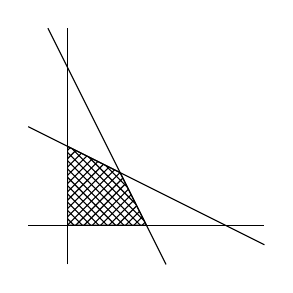
\begin{tikzpicture}
% taralı bölge
\draw [pattern = crosshatch] (0, 0) -- (0, 1) -- (2/3, 2/3) -- (1, 0) -- cycle;
%\draw [pattern = crosshatch] (0, 0) -- (0, 1) -- (2/3, 2/3) -- (1, 0) -- (0, 0); % alternatif yazım
% eksenler
\draw (-0.5, 0) -- (2.5, 0);
\draw (0, -0.5) -- (0, 2.5);
% kısıtlar
\draw (-0.25, 2.5) -- (1.25, -0.5);
\draw (-0.5, 1.25) -- (2.5, -0.25);
\end{tikzpicture}

\bigskip
\hrule
\bigskip

\begingroup
\renewcommand \a {1}
\renewcommand \b {2}
\begin{tikzpicture}[declare function = {
	f(\x) = sqrt(\x);
}]
	\draw (0.5, 0) -- (2.5, 0);
    	\draw [domain = 0.5 : 2.5, samples = 100] plot (\x, {f(\x)}) node [right] {$f$};
    	\filldraw [pattern = north west lines]
    		(\a, 0)
	    	-- plot [domain = \a : \b, samples = 100] (\x, {f(\x)})
	    	-- (\b, 0)
	    	-- cycle;
	% a ve b'nin altının aynı hizada olması için below yerine above
	\node [above] at (\a, -0.5) {$a$};
	\node [above] at (\b, -0.5) {$b$};
\end{tikzpicture}
\endgroup

\newpage

%%%%%%% SAYFA 6 %%%%%%%

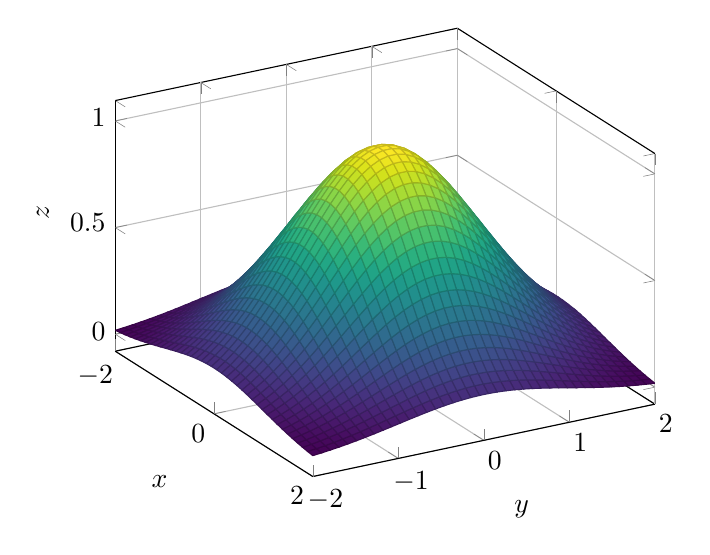
\begin{tikzpicture}
    \begin{axis}[
        xlabel={$x$},
        ylabel={$y$},
        zlabel={$z$},
        colormap/viridis,
        view={60}{30},
        grid=both
    ]
        \addplot3[
            surf,
            domain=-2:2,
            domain y=-2:2,
            samples=40,
            z buffer=sort
        ] {exp(-(x^2 + y^2)/2)};
    \end{axis}
\end{tikzpicture}

\bigskip
\hrule
\bigskip

\begingroup
\renewcommand \pi {3.141593} % pi sayısı
\newcommand \m {6} % ortalama
\newcommand \s {1.897367} % standart sapma
\newcommand \xs {0.75} % x ölçeği
\newcommand \ys {15} % y ölçeği
\begin{tikzpicture}[xscale = \xs, yscale = \ys, declare function = {
	n(\x) = (1 / (sqrt(2*\pi) * \s)) * exp(-0.5 * ((\x - \m) / \s)^2);
}]
	% eksen
	\draw (0, 0) -- (15, 0);
    	\draw (0, -0.05/\ys) grid (15, 0.05/\ys);
	\foreach \i in {0, ..., 15}
		\node [below] at (\i, -0.05/\ys) {\i};	
	% binom olasılık kütle fonksiyonu değerleri
	\foreach \x/\y in {
		0/4.702e-04,
		1/4.702e-03,
		2/2.194e-02,
		3/6.339e-02,
		4/1.268e-01,
		5/1.859e-01,
		6/2.066e-01,
		7/1.771e-01,
		8/1.181e-01,
		9/6.121e-02,
		10/2.449e-02,
		11/7.420e-03,
		12/1.649e-03,
		13/2.537e-04,
		14/2.416e-05,
		15/1.074e-06
        } {
        	\filldraw (\x, \y) ellipse [x radius = 2/\xs pt, y radius = 2/\ys pt];
        }
        % normal yaklaşım	
    	\draw [domain = 0 : 15, samples = 100] plot (\x, {n(\x)});
\end{tikzpicture}
\endgroup

\end{document}